% Esqueleto do relatório (Fase III). Só estrutura: toda a redação é do grupo (regra 4.1 do enunciado).
% Base: abnTeX2 (ABNT). CONFERIR contra o MDT UFSM vigente (margens, fonte, citações, referências).
\documentclass[12pt,a4paper,oneside,brazil]{abntex2}
\usepackage[T1]{fontenc}
\usepackage[utf8]{inputenc}
\usepackage{lmodern,graphicx,booktabs,indentfirst}
\usepackage[brazilian,hyperpageref]{backref}
\usepackage[alf]{abntex2cite}
\graphicspath{{../figuras/}}

\titulo{% TODO: título
}
\autor{% TODO: autores
}
\local{Santa Maria}
\data{2026}
\instituicao{Universidade Federal de Santa Maria}
\preambulo{% TODO: natureza do trabalho, disciplina e professor
}

\begin{document}
\imprimircapa
\imprimirfolhaderosto*

\begin{resumo}
% TODO
\end{resumo}

\pdfbookmark[0]{\listfigurename}{lof}\listoffigures*\cleardoublepage
\pdfbookmark[0]{\listtablename}{lot}\listoftables*\cleardoublepage
\pdfbookmark[0]{\contentsname}{toc}\tableofcontents*\cleardoublepage

\textual

\chapter{Introdução}
% TODO: empresa, problema central, justificativa

\chapter{Embasamento teórico}
\section{IA generativa e LLMs}
% TODO
\section{Sistemas de agente único e multiagentes}
% TODO
\section{Engenharia de prompt, uso de ferramentas e RAG}
% TODO
\section{Métodos de otimização e decisão}
% TODO

% Tabelas prontas em tabelas/*.tex (gerar_tabelas.py): \begin{table}\caption{..}\small\begin{tabular}{llrrl}
\toprule
\textbf{ID} & \textbf{Proposta} & \textbf{Efeito mensal} & \textbf{Efeito pontual} & \textbf{Parecer} \\
\midrule
FIN-1 & Regularizar dividendos: corrente em dia e atrasados em 24 meses & R\$ -991.443 & R\$ 0 & aprovada \\
FIN-2 & Priorizar a entrega dos 27 pedidos pendentes & R\$ 0 & R\$ 7.072.776 & aprovada \\
FIN-3 & Reduzir a produção do elétrico para aliviar caixa (alternativa avaliada) & R\$ 0 & R\$ 0 & reprovada \\
FIN-4 & Revisar a remuneração da diretoria (-20\%) & R\$ 76.610 & R\$ 0 & condicional \\
OPE-1 & Operar em 2 turnos (3º turno só nos picos) e dimensionar o quadro de operadores & R\$ 58.415 & R\$ 0 & condicional \\
OPE-2 & Manutenção preventiva e padrão de trabalho nas etapas 20, 50 e 60 & R\$ 2.156 & R\$ 0 & aprovada \\
SUP-1 & Comprar as peças longas no ato do pedido firme (ar-condicionado 45 d, portas 30 d, inversor 60 d) & R\$ 0 & R\$ 421.092 & aprovada \\
SUP-2 & Cotar alternativas para ar-condicionado (Thermo King) e portas (Bode) & R\$ 0 & R\$ 0 & aprovada \\
SUP-3 & Elétrico só contra pedido firme e negociar pagamento do inversor na entrega & R\$ 0 & R\$ 0 & aprovada \\
MER-1 & Priorizar a venda dos modelos de maior lucro por ônibus (frotas sequenciais para prefeituras) & R\$ 0 & R\$ 0 & aprovada \\
MER-2 & Fase 2: double-deck e novos segmentos & R\$ 0 & R\$ 0 & aprovada \\
\bottomrule
\end{tabular}
\fonte{..}\end{table}
\chapter{Aplicação prática}
\section{Resultados da entrevista}
% TODO: fase1-*.md, respostas-*.md
\section{Arquitetura do sistema}
% TODO: papel de cada agente, ferramentas, regras de validação
\begin{figure}[htb]
  \caption{% TODO
  }
  \centering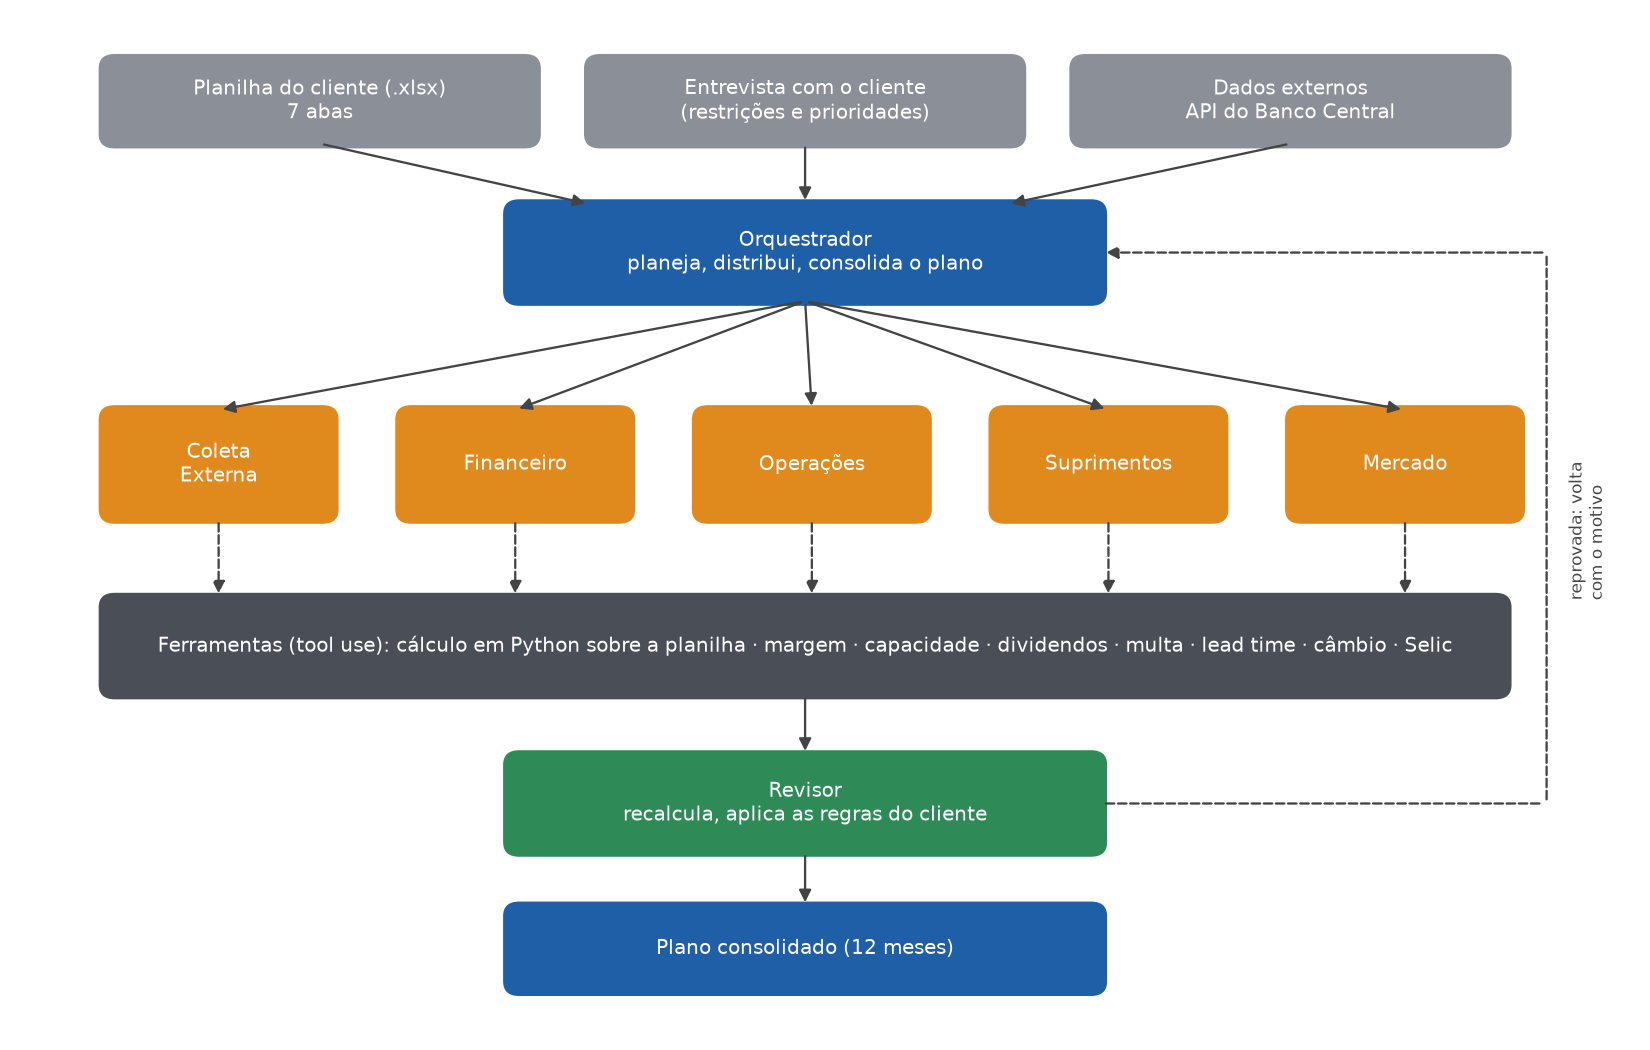
\includegraphics[width=\textwidth]{01_arquitetura.png}
  \fonte{% TODO
  }
\end{figure}

\section{Análise dos dados}
% TODO: margens, carteira, capacidade, refugo, fornecedores (figuras 02 a 06)
\begin{figure}[htb]
  \caption{% TODO
  }
  \centering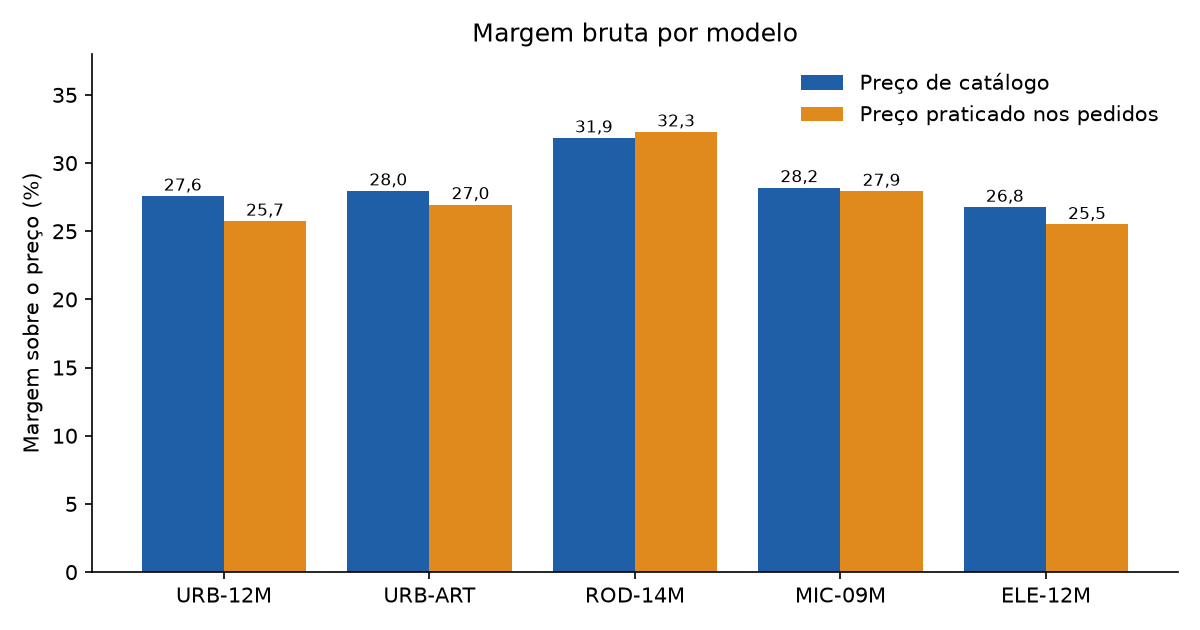
\includegraphics[width=.8\textwidth]{02_margem_modelos.png}
  \fonte{% TODO
  }
\end{figure}
% Demais figuras: 03_carteira_pedidos, 04_capacidade_linha, 05_refugo_etapas, 06_leadtime_pecas

\section{Soluções propostas e impacto}
% TODO: plano-consolidado.md
\begin{figure}[htb]
  \caption{% TODO
  }
  \centering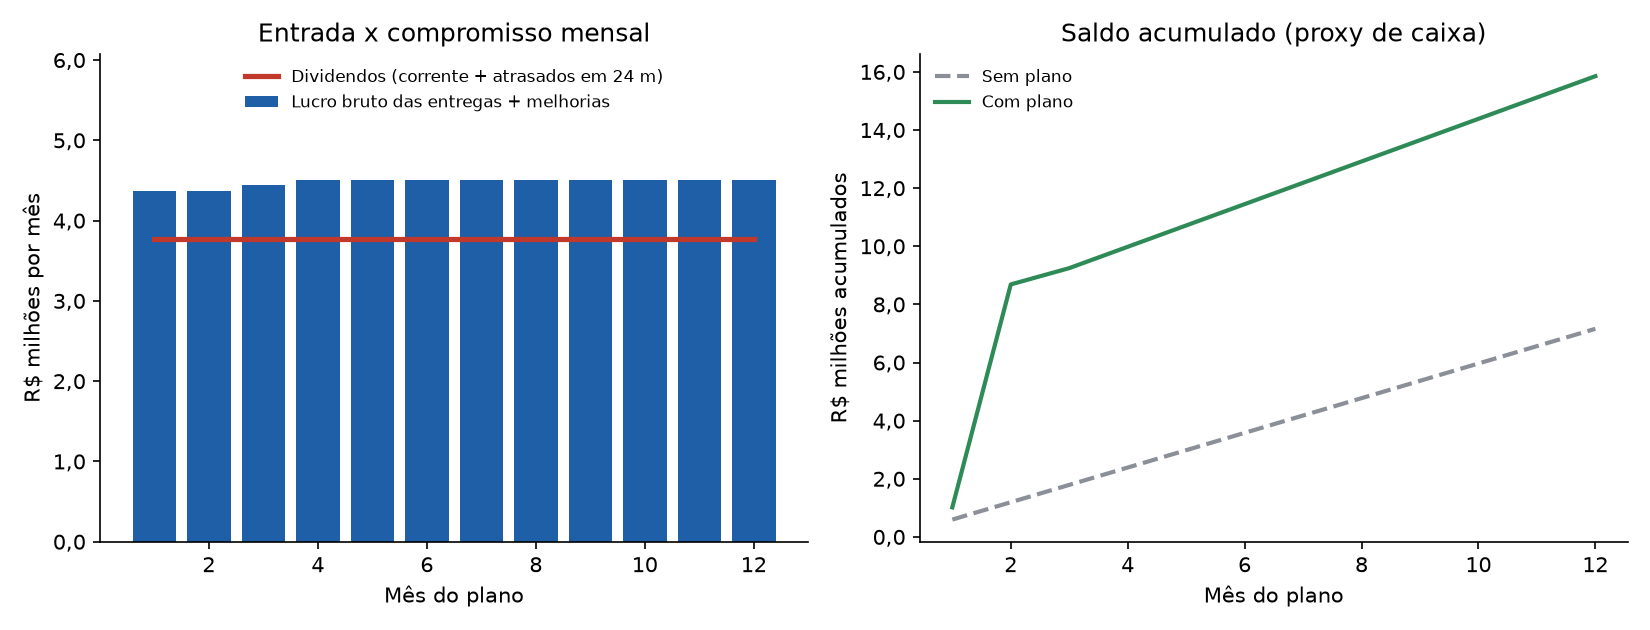
\includegraphics[width=\textwidth]{07_caixa_dividendos.png}
  \fonte{% TODO
  }
\end{figure}

\chapter{Conclusão}
% TODO: síntese, limitações, recomendações

\postextual
\bibliography{referencias}

\end{document}
